% Options for packages loaded elsewhere
\PassOptionsToPackage{unicode}{hyperref}
\PassOptionsToPackage{hyphens}{url}
%
\documentclass[
  12pt,
]{article}
\usepackage{amsmath,amssymb}
\usepackage{lmodern}
\usepackage{iftex}
\ifPDFTeX
  \usepackage[T1]{fontenc}
  \usepackage[utf8]{inputenc}
  \usepackage{textcomp} % provide euro and other symbols
\else % if luatex or xetex
  \usepackage{unicode-math}
  \defaultfontfeatures{Scale=MatchLowercase}
  \defaultfontfeatures[\rmfamily]{Ligatures=TeX,Scale=1}
\fi
% Use upquote if available, for straight quotes in verbatim environments
\IfFileExists{upquote.sty}{\usepackage{upquote}}{}
\IfFileExists{microtype.sty}{% use microtype if available
  \usepackage[]{microtype}
  \UseMicrotypeSet[protrusion]{basicmath} % disable protrusion for tt fonts
}{}
\makeatletter
\@ifundefined{KOMAClassName}{% if non-KOMA class
  \IfFileExists{parskip.sty}{%
    \usepackage{parskip}
  }{% else
    \setlength{\parindent}{0pt}
    \setlength{\parskip}{6pt plus 2pt minus 1pt}}
}{% if KOMA class
  \KOMAoptions{parskip=half}}
\makeatother
\usepackage{xcolor}
\usepackage[margin=1in]{geometry}
\usepackage{graphicx}
\makeatletter
\def\maxwidth{\ifdim\Gin@nat@width>\linewidth\linewidth\else\Gin@nat@width\fi}
\def\maxheight{\ifdim\Gin@nat@height>\textheight\textheight\else\Gin@nat@height\fi}
\makeatother
% Scale images if necessary, so that they will not overflow the page
% margins by default, and it is still possible to overwrite the defaults
% using explicit options in \includegraphics[width, height, ...]{}
\setkeys{Gin}{width=\maxwidth,height=\maxheight,keepaspectratio}
% Set default figure placement to htbp
\makeatletter
\def\fps@figure{htbp}
\makeatother
\setlength{\emergencystretch}{3em} % prevent overfull lines
\providecommand{\tightlist}{%
  \setlength{\itemsep}{0pt}\setlength{\parskip}{0pt}}
\setcounter{secnumdepth}{-\maxdimen} % remove section numbering
\usepackage{fancyhdr}
\usepackage{fontspec}
\usepackage{xcolor}
\usepackage{hyperref}
\usepackage{pdfcomment}
\usepackage{datetime}
\usepackage{subfig}
\usepackage{float}
\usepackage[document]{ragged2e}

\setmainfont{Poppins}

% \fancypagestyle{plain}{\pagestyle{fancy}} % added to show header and footer in the first page

% header and footer
\pagestyle{fancy}
\setlength{\headheight}{75pt}
\setlength{\textheight}{600pt}
\fancyhead[C]{}
\fancyhead[L]{
\includegraphics{X:/DSA/Trends/household-travel-survey/headers/PST_2021_HTS_header.png}}
\fancyhead[R]{}
\newdateformat{monthyeardate}{\monthname[\THEMONTH] \THEYEAR}
\fancyfoot[L]{\scriptsize{1011 Western Ave, Suite 500, Seattle WA 98104} \textcolor[HTML]{F05A28}. 206.464.7532 \textcolor[HTML]{F05A28}. www.psrc.org \textcolor[HTML]{F05A28}. \monthyeardate\today}
\fancyfoot[R]{\textcolor[HTML]{F05A28}\thepage}
\fancyfoot[C]{}
\renewcommand{\headrulewidth}{0pt}
\renewcommand{\footrulewidth}{4pt}
\renewcommand{\footrule}{\hbox to \headwidth{\color[HTML]{BCBEC0}\leaders\hrule height \footrulewidth\hfill}}
\ifLuaTeX
  \usepackage{selnolig}  % disable illegal ligatures
\fi
\IfFileExists{bookmark.sty}{\usepackage{bookmark}}{\usepackage{hyperref}}
\IfFileExists{xurl.sty}{\usepackage{xurl}}{} % add URL line breaks if available
\urlstyle{same} % disable monospaced font for URLs
\hypersetup{
  hidelinks,
  pdfcreator={LaTeX via pandoc}}

\author{}
\date{\vspace{-2.5em}}

\begin{document}

\hypertarget{womens-travel-needs-often-go-overlooked}{%
\section{Women's Travel Needs Often Go
Overlooked}\label{womens-travel-needs-often-go-overlooked}}

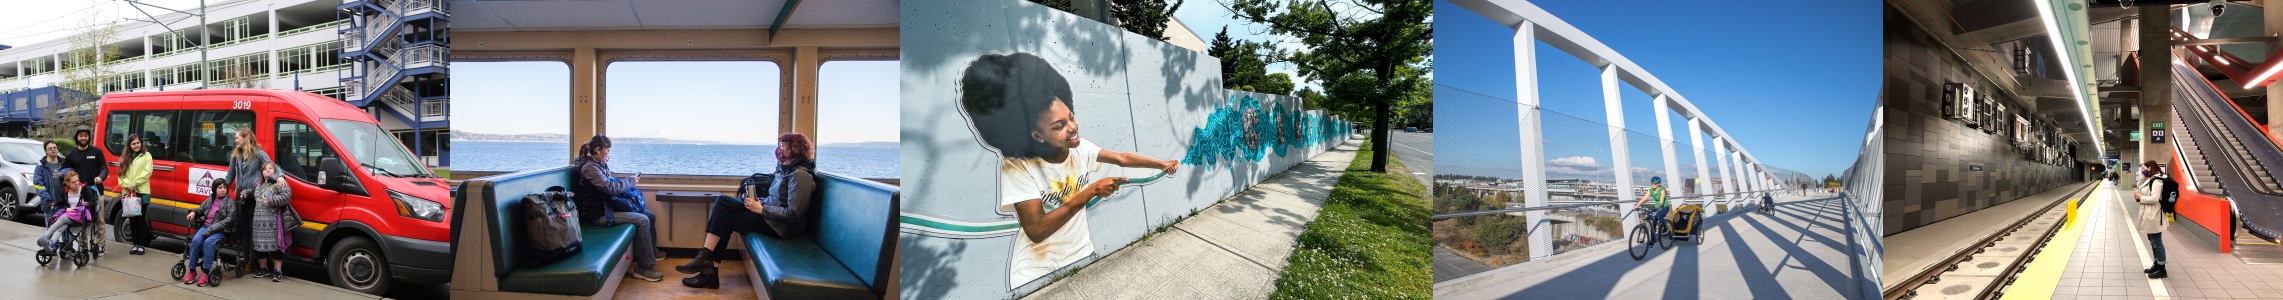
\includegraphics[width=1\textwidth,height=\textheight]{C:/Coding/CURRENT_REPOS_GITHUB/document-maker/templates/equity_example/women2_image_header.png}

\begin{flushleft}
The way in which we design our urban environments oftentimes overlooks the needs of families and female-identifying residents. Leslie Kern's book \href{https://metropolismag.com/viewpoints/leslie-kern-feminist-city/}{\underline{\textcolor{blue}{Feminist City}}} explores some of the ways in which we can redesign and shape our cities through a mor equitable process. \smallskip

One example in particular, is how women have \href{http://libraryarchives.metro.net/DB_Attachments/2019-0294/UnderstandingHowWomenTravel_FullReport_FINAL.pdf}{\underline{\textcolor{blue}{transportation needs that have not historically been met}}} in urban environments. The regional transportation system (including transit) was traditionally designed around the need to quickly get to work at central locations. Women tend to carry significantly more of the care-giving burdens of society and thus need a system that works \textbf{safely} for traveling with others to a variety of locations \textbf{at all times of day}. Women also represent a large portion of older populations who have unique transportation needs that are not well-served by our system built around driving and work destinations. Furthermore, women are more likely to live in poverty and have lower incomes than men, which impact many aspects of transit needs and housing needs or limitations. (Read our Equity Trend story from last year about \href{https://www.psrc.org/about-us/media-hub/womens-history-month-progress-and-paychecks}{\underline{\textcolor{blue}{Women's History Month: progress and paychecks}}} for gendered income disparities). \smallskip

With the arrival of the COVID-19 pandemic, we saw a greater trend towards telecommuting for some people and continued trends in aging. With these new considerations at play, compounded with the existence on previous burdens on women, when will the transportation system evolve for women?
\end{flushleft}

\newpage
\setlength{\headheight}{10pt}
\setlength{\textheight}{665pt}
\fancyhead[L]{}

\hypertarget{puget-sound-regional-household-travel-survey}{%
\section{Puget Sound Regional Household Travel
Survey}\label{puget-sound-regional-household-travel-survey}}

\begin{flushleft}
The 2017, 2019, and 2021 household travel surveys collected day-to-day information from households in the central Puget Sound region, such as how we traveled, where we went, how long it took—even where we chose to live and whether we got home deliveries, prior to COVID-19 and after. \smallskip


This report starts with comparing travel by gender, during the stable period prior to COVID-19, and then dives into some broader, national trends, and finishes by taking a glance at recent trends that occurred in 2021, during COVId-19.  Learn more at the \href{https://www.psrc.org/our-work/household-travel-survey-program}{\underline{\textcolor{blue}{household travel survey webpage}}}. Data from 2017 and 2019 have combined to give a more robust sample size.  You can also \href{https://household-travel-survey-psregcncl.hub.arcgis.com}{\underline{\textcolor{blue}{view the full dataset here}}}, including 2017, 2019 and 2021 data. 
\end{flushleft}

\hypertarget{travel-behavior-and-transit-trends}{%
\subsection{Travel Behavior and Transit
Trends}\label{travel-behavior-and-transit-trends}}

\begin{flushleft}
Through the analysis in this report, key trends have emerged that differentiate female-identifying resident’s travel patterns from men’s travel patterns, across all modes. Across all modes, more women are making many more trips \textbf{(7 or more)} per day than men. Inversely, more women than men are also not making any trips per day. This means women may experience more exposure to travel burdens (cost, stress, or safety risks), or may be more likely to be isolated or disconnected from the opportunities that travel affords. They exist more frequently on both sides of the spectrum.

Womens' trips are more varied to a broader spread of destinations, and are more likely to primarily serve the needs of someone else (Figure 1). Women are more likely to live in a car-free or car-light household, take more trips with other people, take fewer single-occupant car trips than men, and are more likely to carpool or get a ride from a family member or friend if they don’t have a driver’s license. 
\end{flushleft}

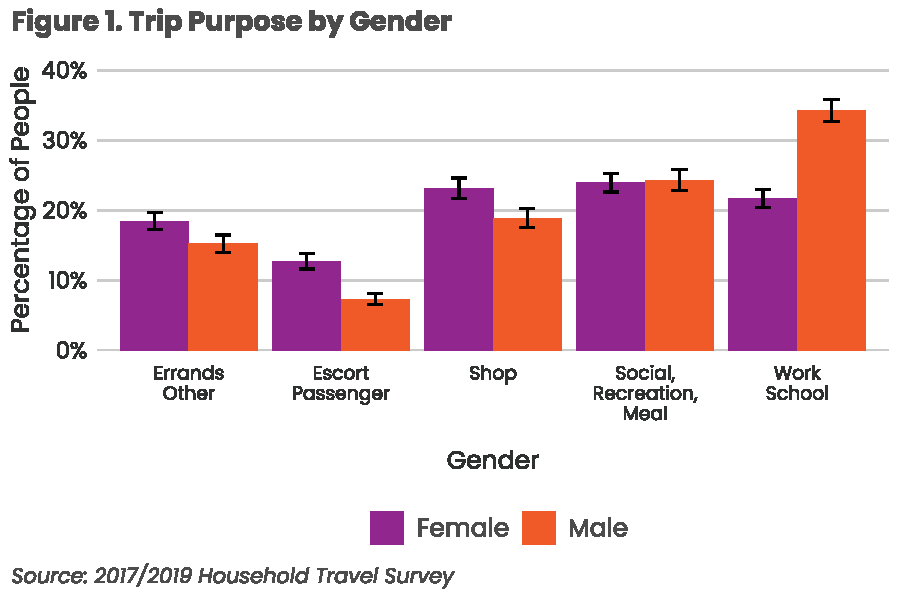
\includegraphics{womens_history_story_draft_files/figure-latex/trip by gender-1.pdf}

\begin{flushleft}
Women in households with more than two people tend to travel more with other people than men (Figure 2). Transit is often not well set up for people who are traveling with strollers. The walk and bike network are not built out for people of all ages to use.
\end{flushleft}

\hypertarget{transit-isnt-always-efficient-for-women}{%
\subsubsection{Transit isn't Always Efficient for
Women}\label{transit-isnt-always-efficient-for-women}}

\begin{flushleft}
Among female transit riders, almost 90\% ride the system more than three days per week. Fifty-seven percent of women bring their children on transit, and they often ride transit because they do not have a car, they want to avoid traffic, or because they do not have a license. Two of these three reasons indicate that women who ride transit do so because they have fewer transportation options, and may have less access to economic opportunities as a result. Over 85\% of women riders use Metro to travel to work or school, and of those women, 32\% also use Metro to run errands or complete recreational trips. Among people who make household serving trips most frequently, these trips comprise the same share for women whether they use transit or not; for men, the share of household-serving trips declines if they are transit users. This shows that while men are more likely to find alternatives to using transit to complete household-serving trips (using a different mode or taking fewer trips), women are less likely to find an alternative, and instead work to make the transit system work for their needs. Although the rate of adoption for Transportation Network Companies (TNCs) like Uber and Lyft is the same for men and women, women are more likely than men to report that their transit use has stayed the same as they have also begun to use TNCs. Women are more likely than men to say they use TNCs for trips that transit does not serve, while men are more likely to say they use TNCs to reach a transit stop or station. The trips that are not served by transit may be related to time or location, as women’s needs differ from men’s needs by both time of day and location.
\end{flushleft}

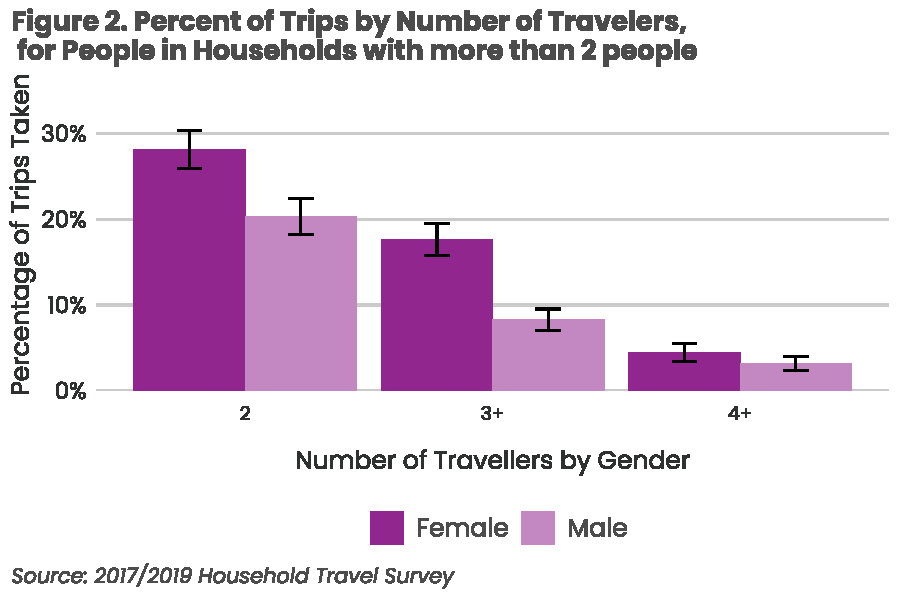
\includegraphics{womens_history_story_draft_files/figure-latex/Trips by Number of Travellers-1.pdf}
\newpage \setlength{\headheight}{10pt} \setlength{\textheight}{665pt}
\fancyhead[L]{}

\hypertarget{transportation-modalities}{%
\subsection{Transportation Modalities}\label{transportation-modalities}}

\hypertarget{women-bike-commute-far-less-than-men}{%
\subsubsection{Women Bike Commute Far Less than
Men}\label{women-bike-commute-far-less-than-men}}

\begin{flushleft}
Women bike much less than men. Some of this is undoubtedly because of bike network design does not feel well-suited or safe for all people of different ages and abilities. There are many considerations as to why women do not feel comfortable riding bicycles as a form of transit, as seen in a study performed by the \href{https://www.itdp.org/2022/07/06/cyclings-gender-gap/}{\underline{\textcolor{blue}{Institute for Transportation and Development Policy}}} in 2022. The inclusion of designated bike lanes, not only that increase comfort and safety for individuals, but that make traveling with children or larger cargo bikes easier would help create more accessibility and user-friendly options. Additionally, increased education about bike routes and access to bikes as a means to developing a biker's comfort and familiarity with bike safety, would help aid in bike commuting ease. 

As a result of some of these considerations not being implemented, in the Puget Sound Region in 2019 only \textbf{6,000} bike trips were made by non-binary folks, and \textbf{30,000} bike trips were made by women, but \textbf{74,000} were made by men (Figure 3). 
\end{flushleft}

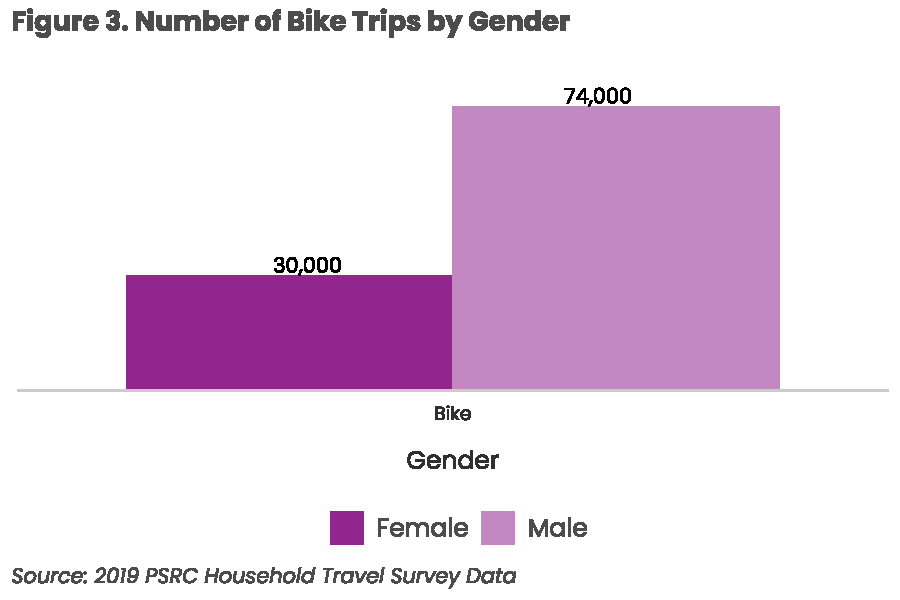
\includegraphics{womens_history_story_draft_files/figure-latex/Bike trips-1.pdf}

\begin{flushleft}
Not only are certain modalities not conducive to ways in which women move abou their environment, but there is also the concern for safety. \href{https://www.itdp.org/2022/07/06/cyclings-gender-gap/}{\underline{\textcolor{blue}{The Institute for Transportation and Development Policy in 2022}}} reported that even though women chose biking less often then men, there was still an active participation in dialogues about how to increase user uptake and accessibility with biking because they deemed it a way to remain safe from harassment or negative transit or walking encounters that they experienced. Women should not have to choose between safety concerns.

How can the transportation and land use system better accommodate older people, household maintenance and caregiving needs? Addressing these questions will improve the system for all genders.
\end{flushleft}

\newpage
\setlength{\headheight}{10pt}
\setlength{\textheight}{665pt}
\fancyhead[L]{}

\hypertarget{implications-for-womens-limitations-and-accessibility}{%
\subsection{Implications for Women's Limitations and
Accessibility}\label{implications-for-womens-limitations-and-accessibility}}

\begin{flushleft}
Household Travel Survey Data from 2017 and 2019 combined suggest that women make more trips for care-giving purposes like escorting passengers, shopping, running household errands, and less trips for work and school.

These findings suggest that women are required to adjust their own schedule and travel needs to accommodate others, and in doing so, give up some of their own autonomy and control over when and how they travel. Despite these challenges and tradeoffs, women show ingenuity in arranging their schedules to meet their travel needs. Women are more likely to trip-chain, or make stops along the way to other destinations, and describe consolidating all their errand trips into one day where they will have access to a vehicle.

These travel behavior findings point towards many opportunities to adjust the services provided by Metro to better meet the travel needs expressed by those who are using transit. Development of a Gender Action Plan - or a tactical plan to implement policy, design, and service changes throughout the agency - wouldn help to articulate the immediate opportunities and long-term goals that would create a system that better serves women. Adjustments to services, vehicle design, and policy would help minimize the time, cost, safety, and physical burdens and additional emotional labor of riding transit for the more than half of all riders who are women. Gemma Hartley's book speaks to this added level of acrobatics that women oftentimes face when navigating caretaking, professional, and personal hurdles in \href{https://www.gemmahartley.com/}{\underline{\textcolor{blue}{Fed Up: Emotional Labor, Women and the Way Forward}}}.
\end{flushleft}

\newpage
\setlength{\headheight}{10pt}
\setlength{\textheight}{665pt}
\fancyhead[L]{}

\hypertarget{regional-and-nationwide-data-show-similar-constraints}{%
\subsection{Regional and Nationwide Data Show Similar
Constraints}\label{regional-and-nationwide-data-show-similar-constraints}}

\begin{flushleft}
The findings from \href{https://thesource.metro.net/2019/09/19/metro-releases-understanding-how-women-travel-report/}{\underline{\textcolor{blue}{Understanding How Women Travel}}} about women’s mode choices, how likely they are to travel with others in their care, and their complex trip-chaining patterns could all inform adjustments to Metro’s fare policy to make it more equitable towards women and more cost-competitive with driving and carpooling. Findings about women’s trip purposes and primary responsibility for household errands could all inform the way transit vehicles, transit stations, and bus stops are designed, so that space for traveling with others and carrying  belongings could be better accommodated. Findings about when women are traveling and average trip lengths could inform new service offerings that meet a mid-day peak travel demand and provide better direct connections over long distances while minimizing transfers. Women take shorter more local trips, as opposed to long highway trips (Figure 4).
\end{flushleft}

\includegraphics{womens_history_story_draft_files/figure-latex/trip distance by gender-1.pdf}

\begin{flushleft}
Another reason for some of these trip disparities and distance differences is that PUMS data shows men are employed more than women. As we consider the intersectionality of race, gender, and employment, although gendered differences don't appear to be great between races, the disparity amongst men and women across People of Color and white residents is greater (\textbf{10% compared to 8%}). The transportation system needs to be set up for people getting to a variety of locations by a variety of modes, and one that addresses the needs of all income levels.
\end{flushleft}

\includegraphics[height=0.8\textheight]{womens_history_story_draft_files/figure-latex/matrix-1}
\includegraphics[height=0.8\textheight]{womens_history_story_draft_files/figure-latex/matrix-2}

\begin{flushleft}
Another consideration for amending transit and transportation access is that, women, on average, tend to live longer than men, so that at older ages there are many more women who have unique travel needs than men (Figure 6). Women represent a greater share of the older population who needs more specialized transportation services, and less service to work locations. \href{https://www.nytimes.com/2022/12/03/health/elderly-living-alone.html}{\underline{\textcolor{blue}{New York Times}}}.  Older people (who tend to be women more often) have more need for transit in off-peak hours and specialized transportation services. 
\end{flushleft}

\includegraphics{womens_history_story_draft_files/figure-latex/Age group by gender-1.pdf}

\newpage
\setlength{\headheight}{10pt}
\setlength{\textheight}{665pt}
\fancyhead[L]{}

\hypertarget{changes-brought-about-by-covid-19-pandemic}{%
\subsection{Changes Brought about by COVID-19
Pandemic}\label{changes-brought-about-by-covid-19-pandemic}}

\begin{flushleft}
Although there were apparent disparities in the 2017/2019 data, COVID-19 brought about abrupt changes to the transportation landscape in 2021. The 2021 Household Travel survey showed big changes in travel behavior. More people were walking and biking, and less people were using transit. Many more people also now had the opportunity to telework. Although women teleworked more than men before COVID-19, the data shows this increase \textbf{even more in 2021}. In 2021, 41\% of women teleworked, as compared to 33\% of men (Figure 7). The difference between telework rates relates to women's job sectors as compared to men, and also household responsibilities.
\end{flushleft}

\includegraphics{womens_history_story_draft_files/figure-latex/2017/2019 to 2021 charts-1.pdf}

\hypertarget{trip-purpose-by-gender-20172019-to-2021}{%
\subsection{Trip Purpose by Gender (2017/2019 to
2021)}\label{trip-purpose-by-gender-20172019-to-2021}}

\begin{flushleft}
Not only were there changes in the trips made to work for men and women, but overall trip purpose changed from 2017/2019 to 2021 (Figure 8). COVID-19 brought about an increase in social, recreational, or restaurant/meal pick-ups in 2021 for both men and women, but with women surpassing men in percentage of these trips made. Additionally, although it appeared as though women made less trips escorting additional family members (\textbf{from 13% to 8%}), men's trips remained at \textbf{~7%}, which means that overall trips changed, possibly due to the increase in women's telecommute behaviors or lack of activities outside of the home. Overall, women made more trips than men in all other categories besides work or school trips. 
\end{flushleft}

\includegraphics{womens_history_story_draft_files/figure-latex/2017/2019 to 2021-1.pdf}

\newpage
\setlength{\headheight}{10pt}
\setlength{\textheight}{665pt}
\fancyhead[L]{}

\hypertarget{conclusion}{%
\subsection{Conclusion}\label{conclusion}}

\begin{flushleft}
someotherwords
\end{flushleft}

\hypertarget{while-we-are-working-towards-a-more-non-binary-understand-of-gendered-data-we-acknowledge-that-much-of-the-data-presented-above-does-analyze-information-and-patterns-in-a-binary-manner.}{%
\paragraph{While we are working towards a more non-binary understand of
gendered data, we acknowledge that much of the data presented above does
analyze information and patterns in a binary
manner.}\label{while-we-are-working-towards-a-more-non-binary-understand-of-gendered-data-we-acknowledge-that-much-of-the-data-presented-above-does-analyze-information-and-patterns-in-a-binary-manner.}}

\end{document}
